\documentclass{beamer}
% Load csquotes for the \enquote command
\usepackage{csquotes}
\usepackage{hyperref}
\usepackage{nicefrac}
% Load biblatex for bibliography management
\usepackage[backend=biber, style=authoryear]{biblatex}
\addbibresource{bibliography.bib} % Specify your BibTeX bibliography file

\mode<presentation> {
\usetheme{CambridgeUS}
\usecolortheme{seahorse}
}

\title{Macroéconomie 1}
\author{Mart\'in Valdez}
\date{IE1}

\begin{document}

\begin{frame}
\titlepage
\end{frame}

% \begin{frame}
% \frametitle{Overview}
% \tableofcontents
% \end{frame}


%-------------------------------------------------
%  Augmented Solow Model
%-------------------------------------------------

\section{Modèle de Solow Augmenté}

\begin{frame}
    \frametitle{Modèle de Solow Augmenté}
    \framesubtitle{Motivation}
    \hypertarget{augmented_solow}{} % Label for hyperlinks
    Le modèle de Solow de base présente un problème majeur :

    Le capital et la production par travailleur n'ont pas de croissance constante.
    
    \hyperlink{growth}{Production \beamergotobutton{Graphique}}
    \hyperlink{capital}{Capital \beamergotobutton{Graphique}}
    \hyperlink{wages}{Salaires \beamergotobutton{Graphique}}
    \hyperlink{capital_output_ratio}{Rapport Capital-Production\beamergotobutton{Graphique}}

\end{frame}

\begin{frame}
    \frametitle{Modèle de Solow Augmenté}
    \framesubtitle{Fonction de Production}

    \begin{itemize}
        \item Fonction de production :
        \[
        Y_t = A F(K_t, Z_t N_t)
        \]
        \pause
        \item \( Z_t \) : productivité augmentant le travail
        \item \( Z_t N_t \) : unités d'efficacité du travail
        \pause
        \item Supposons que \( Z_t \) et \( N_t \) croissent avec le temps (valeurs initiales en période 0 normalisées à 1) :
            \begin{align*}
                Z_t &= (1 + z)^t \\
                N_t &= (1 + n)^t
            \end{align*}
        \item Question :\(Z_{t+1} = ?\)
    \end{itemize}
\end{frame}

\begin{frame}
    \frametitle{Variables par Capita et par Unité d'Efficacité}
    \framesubtitle{}

    \begin{itemize}
        \item Définissons \( \hat{k}_t = \frac{K_t}{Z_t N_t} \) et de manière similaire pour les autres variables.
        \pause
        \item Variables en minuscule : par capita.\pause
        \item Variables en minuscule avec "chapeaux" : par unité d'efficacité.\pause
        \item On peut montrer que l'équation centrale modifiée du modèle est :
        \[
        \hat{k}_{t+1} = \frac{1}{(1 + z)(1 + n)} \left[ s A_t f(\hat{k}_t) + (1 - \delta) \hat{k}_t \right]
        \]
        \item Même système qu'avant, multiplié par une constante \( \frac{1}{(1 + z)(1 + n)} \).
    \end{itemize}
\end{frame}

\begin{frame}
    \frametitle{État Stationnaire Augmenté}
    \framesubtitle{}

    \begin{figure}
        \centering
        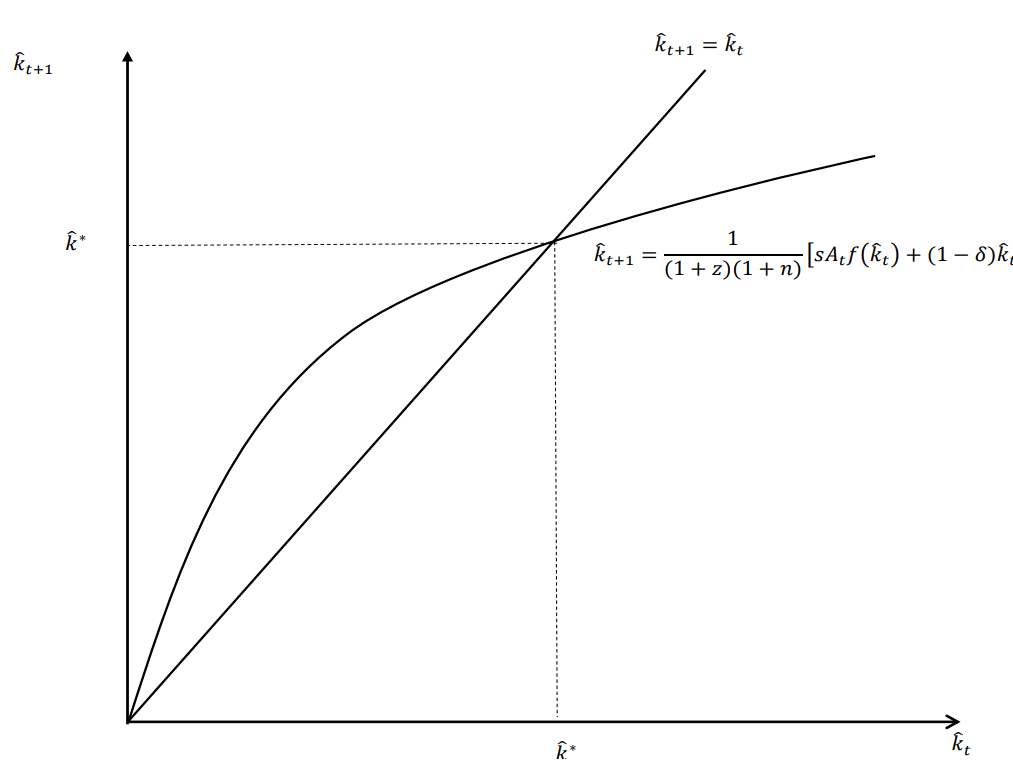
\includegraphics[width=0.8\textwidth]{graphs/ss_solow_s3.png} % Update with the actual path
        \caption{Graphique de l'État Stationnaire Augmenté}
    \end{figure}
\end{frame}

\begin{frame}
    \frametitle{Point d'Équilibre et Taux de Croissance}
    \framesubtitle{}

    \begin{itemize}
        \item Par un raisonnement similaire, le point d'équilibre du système est donné par \( \hat{k}_{t+1} = \hat{k}_t \).
        \item Dans ce nouvel état stationnaire, le stock de capital \( K_t \) croît à un taux de \((1+z)(1+n) \approx z + n\), et
        \item \( k_t \) croît à un taux de \( z \).
    \end{itemize}
\end{frame}

\begin{frame}
    \frametitle{État Stationnaire et Faits de Kaldor}
    \framesubtitle{}

    \begin{itemize}
        \item À l'état stationnaire, nous avons les relations suivantes :
    \end{itemize}

    \[
    \frac{y_{t+1}}{y_t} = 1 + z
    \]
    \[
    \frac{\hat{k}_{t+1}}{\hat{k}_t} = 1 + z
    \]
    \[
    \frac{K_{t+1}}{Y_{t+1}} = \frac{K_t}{Y_t}
    \]
    \[
    \frac{w_{t+1} N_{t+1}}{Y_{t+1}} = \frac{w_t N_t}{Y_t}
    \]
    \[
    R_{t+1} = R_t
    \]
    \[
    \frac{w_{t+1}}{w_t} = 1 + z
    \]

    \begin{itemize}
        \item Ce qui correspond aux six faits de Kaldor !
    \end{itemize}
\end{frame}

\section*{Consommation }

\begin{frame}
    \frametitle{Modèle de Consommation }
    \framesubtitle{Motivation pour un Modèle de Consommation Intertemporelle}

    \begin{itemize}
        \item Dans le modèle de Solow, la consommation est fixe et n'est pas le résultat d'un 
        comportement intertemporel des consommateurs.
        \pause
        \item Il est essentiel de développer un modèle qui capture les décisions de consommation 
        des individus à travers le temps.
        \pause
        \item Un tel modèle nous permettrait de mieux comprendre comment les consommateurs choisissent 
        de répartir leur consommation entre le présent et le futur.
    \end{itemize}
\end{frame}
\begin{frame}
    \frametitle{Pourquoi un Modèle de Consommation ?}
    \framesubtitle{}

    \begin{itemize}
        \item \textbf{Critique de Lucas :} Les modèles doivent intégrer les comportements microéconomiques 
        pour être crédibles et robustes face aux changements du monde réel.
        \pause
        \item Il est crucial de développer une \textbf{théorie} de la consommation pour comprendre les 
        décisions des consommateurs.
        \pause
        \item Nous n'aurons pas le temps de plonger profondément dans cette théorie, mais nous allons examiner 
        rapidement un modèle à deux périodes pour illustrer l'idée.
    \end{itemize}
\end{frame}

\begin{frame}
    \frametitle{Modèle à Deux Périodes}
    \framesubtitle{}

    \begin{itemize}
        \item \textbf{Période 1:} Consommation \( C_1 \), Revenu \( Y_1 \), Épargne \( S \)
        \pause
        \item \textbf{Période 2:} Consommation \( C_2 \), Revenu \( Y_2 \), Retour sur l'épargne \( (1 + r)S \)
        \pause
        \item Les consommateurs choisissent \( C_1 \) et \( C_2 \) pour maximiser leur utilité intertemporelle :
        \[
        U = u(C_1) + \beta u(C_2)
        \]
        Où \( \beta \in (0,1) \) est le taux de préférence temporelle (impatience).
        \item Sous les contraintes budgétaires :
        \begin{align*}
            &C_1 + S = Y_1
            \\
            &C_2 = (1 + r)S + Y_2    
        \end{align*}
        \pause

        \item La solution est une équation appelée \textbf{équation d'Euler}, qui relie la consommation d'aujourd'hui à celle de demain.
    \end{itemize}
\end{frame}

\begin{frame}
    \frametitle{La Fonction de Consommation}
    \framesubtitle{}

    \begin{itemize}
        \item L'équation d'Euler relie la consommation d'aujourd'hui \( C_1 \) à celle de demain \( C_2 \) :
        \[
        u'(C_1) = \beta (1 + r) u'(C_2)
        \]
        Comment y arriver ?
        \pause
        \item Cela permet de définir une fonction de consommation qui donne la consommation d'aujourd'hui en 
        fonction du revenu d'aujourd'hui et du revenu de demain.
        \[
        C_1 = f(Y_1,Y_2) = \frac{1}{1 + \beta} \left[ Y_1 + \frac{1}{1 + r} Y_2 \right] 
        \]
        \item Consommation en fonction de leurs attentes concernant le revenu futur, le taux d'intérêt et leur 
        taux de préférence temporelle.
    \end{itemize}

\end{frame}


\begin{frame}
    \frametitle{Conclusion et Points Clés}

    \begin{itemize}
        \item Arrêtons-nous ici, c'est assez d'informations pour le cours.
        \pause
        \item \textbf{Résumé de notre cours:}
            \begin{itemize}
                \item \textbf{Qu'est-ce que la Macroeconomie?} 
                \begin{itemize}
                    \item L'étude de l'activité économique agrégée.
                \end{itemize}
                \pause
                \item \textbf{Définitions Clés:}
                \begin{itemize}
                    \item Qu'est-ce que le PIB?
                \end{itemize}
                \pause
                \item \textbf{Importance des Modèles:}
                \begin{itemize}
                    \item Pourquoi Utiliser des Modèles?
                \end{itemize}
            \end{itemize}
    \end{itemize}
\end{frame}

\begin{frame}
    \frametitle{Résumé des Modèles et Théories Clés}

    \begin{itemize}
        \item \textbf{Les Faits de Kaldor:}
        \begin{itemize}
            \item Croissance soutenue de la production, du capital et des salaires.
            \item Stabilité du ratio K/Y et du rapport revenu du travail/revenu total wL/Y.
        \end{itemize}
        \pause
        \item \textbf{Le Modèle de Solow:}
        \begin{itemize}
            \item Modèle simple capturant certains faits de Kaldor.
            \item Rôle de la productivité dans la croissance.
        \end{itemize}
        \pause
        \item \textbf{Le Modèle de Solow Augmenté:}
        \begin{itemize}
            \item Intégration de la croissance soutenue dans le modèle de Solow.
        \end{itemize}
        \pause
        \item \textbf{Théorie de la Consommation:}
        \begin{itemize}
            \item Vue rapide sur la théorie microéconomique de la consommation.
        \end{itemize}
    \end{itemize}
\end{frame}


%

%-------------------------------------------------
%  Graphs
%-------------------------------------------------



\begin{frame}
    \frametitle{Kaldor's Stylized Facts}
    \hypertarget{growth}{} % Label for hyperlinks
    \framesubtitle{Croissance de la Production}
        \begin{figure}
            \centering
            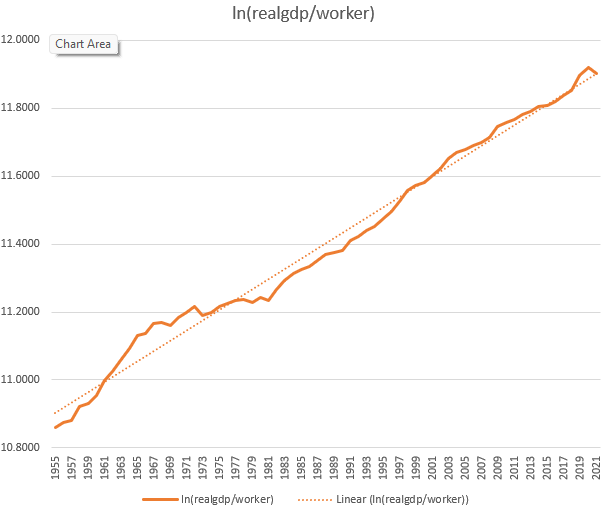
\includegraphics[width=0.6\textwidth]{graphs/lnrgdp_usa.png}
            \caption{Real GDP per Worker, US Economy
            \hyperlink{augmented_solow}{\beamergotobutton{Retour}}}
        \end{figure}
\end{frame}

\begin{frame}
    \frametitle{Kaldor's Stylized Facts}
    \hypertarget{capital}{} % Label for hyperlinks
    \framesubtitle{Accumulation de Capital}
        \begin{figure}
            \centering
            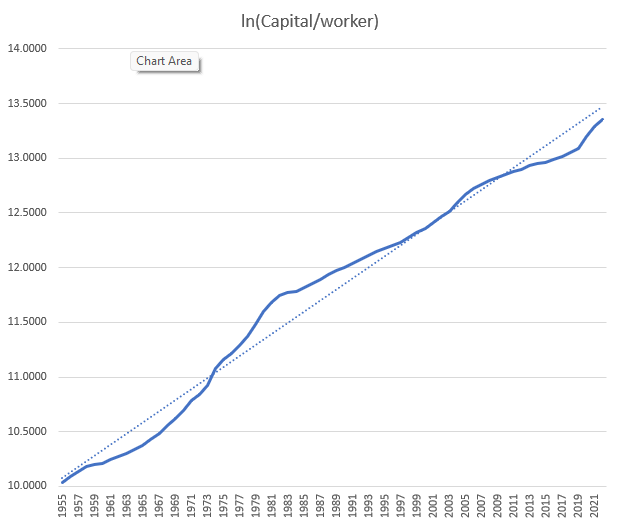
\includegraphics[width=0.6\textwidth]{graphs/lnkperworker_usa.png}
            \caption{Capital per Worker, US Economy
            \hyperlink{augmented_solow}{\beamergotobutton{Retour}}}
        \end{figure}
\end{frame}

\begin{frame}
    \frametitle{Kaldor's Stylized Facts}
    \hypertarget{capital_output_ratio}{} % Label for hyperlinks
    \framesubtitle{Ratio Capital-Production}
        \begin{figure}
            \centering
            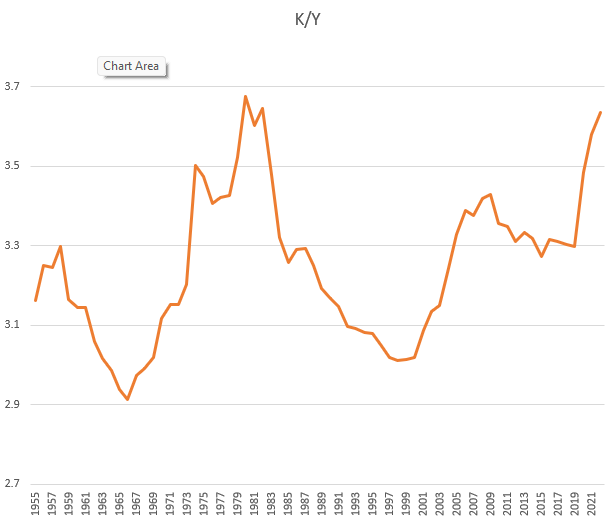
\includegraphics[width=0.55\textwidth]{graphs/kyratio_usa.png}
            \caption{\enquote*{Stability} of Capital-Output Ratio, US Economy
            \hyperlink{augmented_solow}{\beamergotobutton{Retour}}}
        \end{figure}
        
\end{frame}


\begin{frame}
    \frametitle{Kaldor's Stylized Facts}
    \hypertarget{income}{} % Label for hyperlinks
    \framesubtitle{Répartition du Revenu}
        \begin{figure}
            \centering
            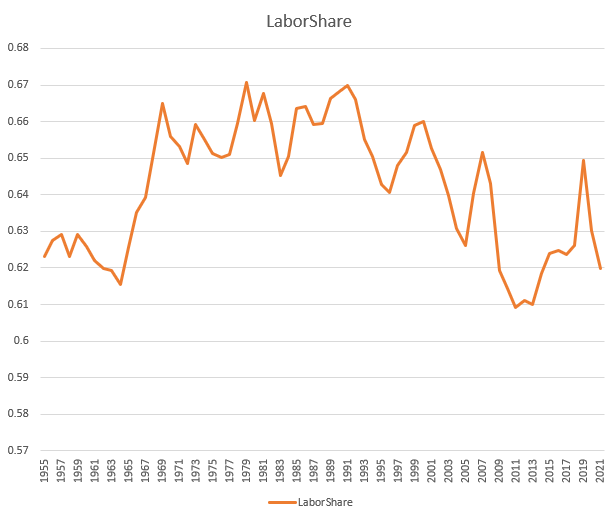
\includegraphics[width=0.6\textwidth]{graphs/labor_share.png}
            \caption{Labour Share of Income, US Economy
            \hyperlink{augmented_solow}{\beamergotobutton{Retour}}}
        \end{figure}
\end{frame}

\begin{frame}
    \frametitle{Kaldor's Stylized Facts}
    \hypertarget{return}{} % Label for hyperlinks
    \framesubtitle{Taux de Rendement}
        \begin{figure}
            \centering
            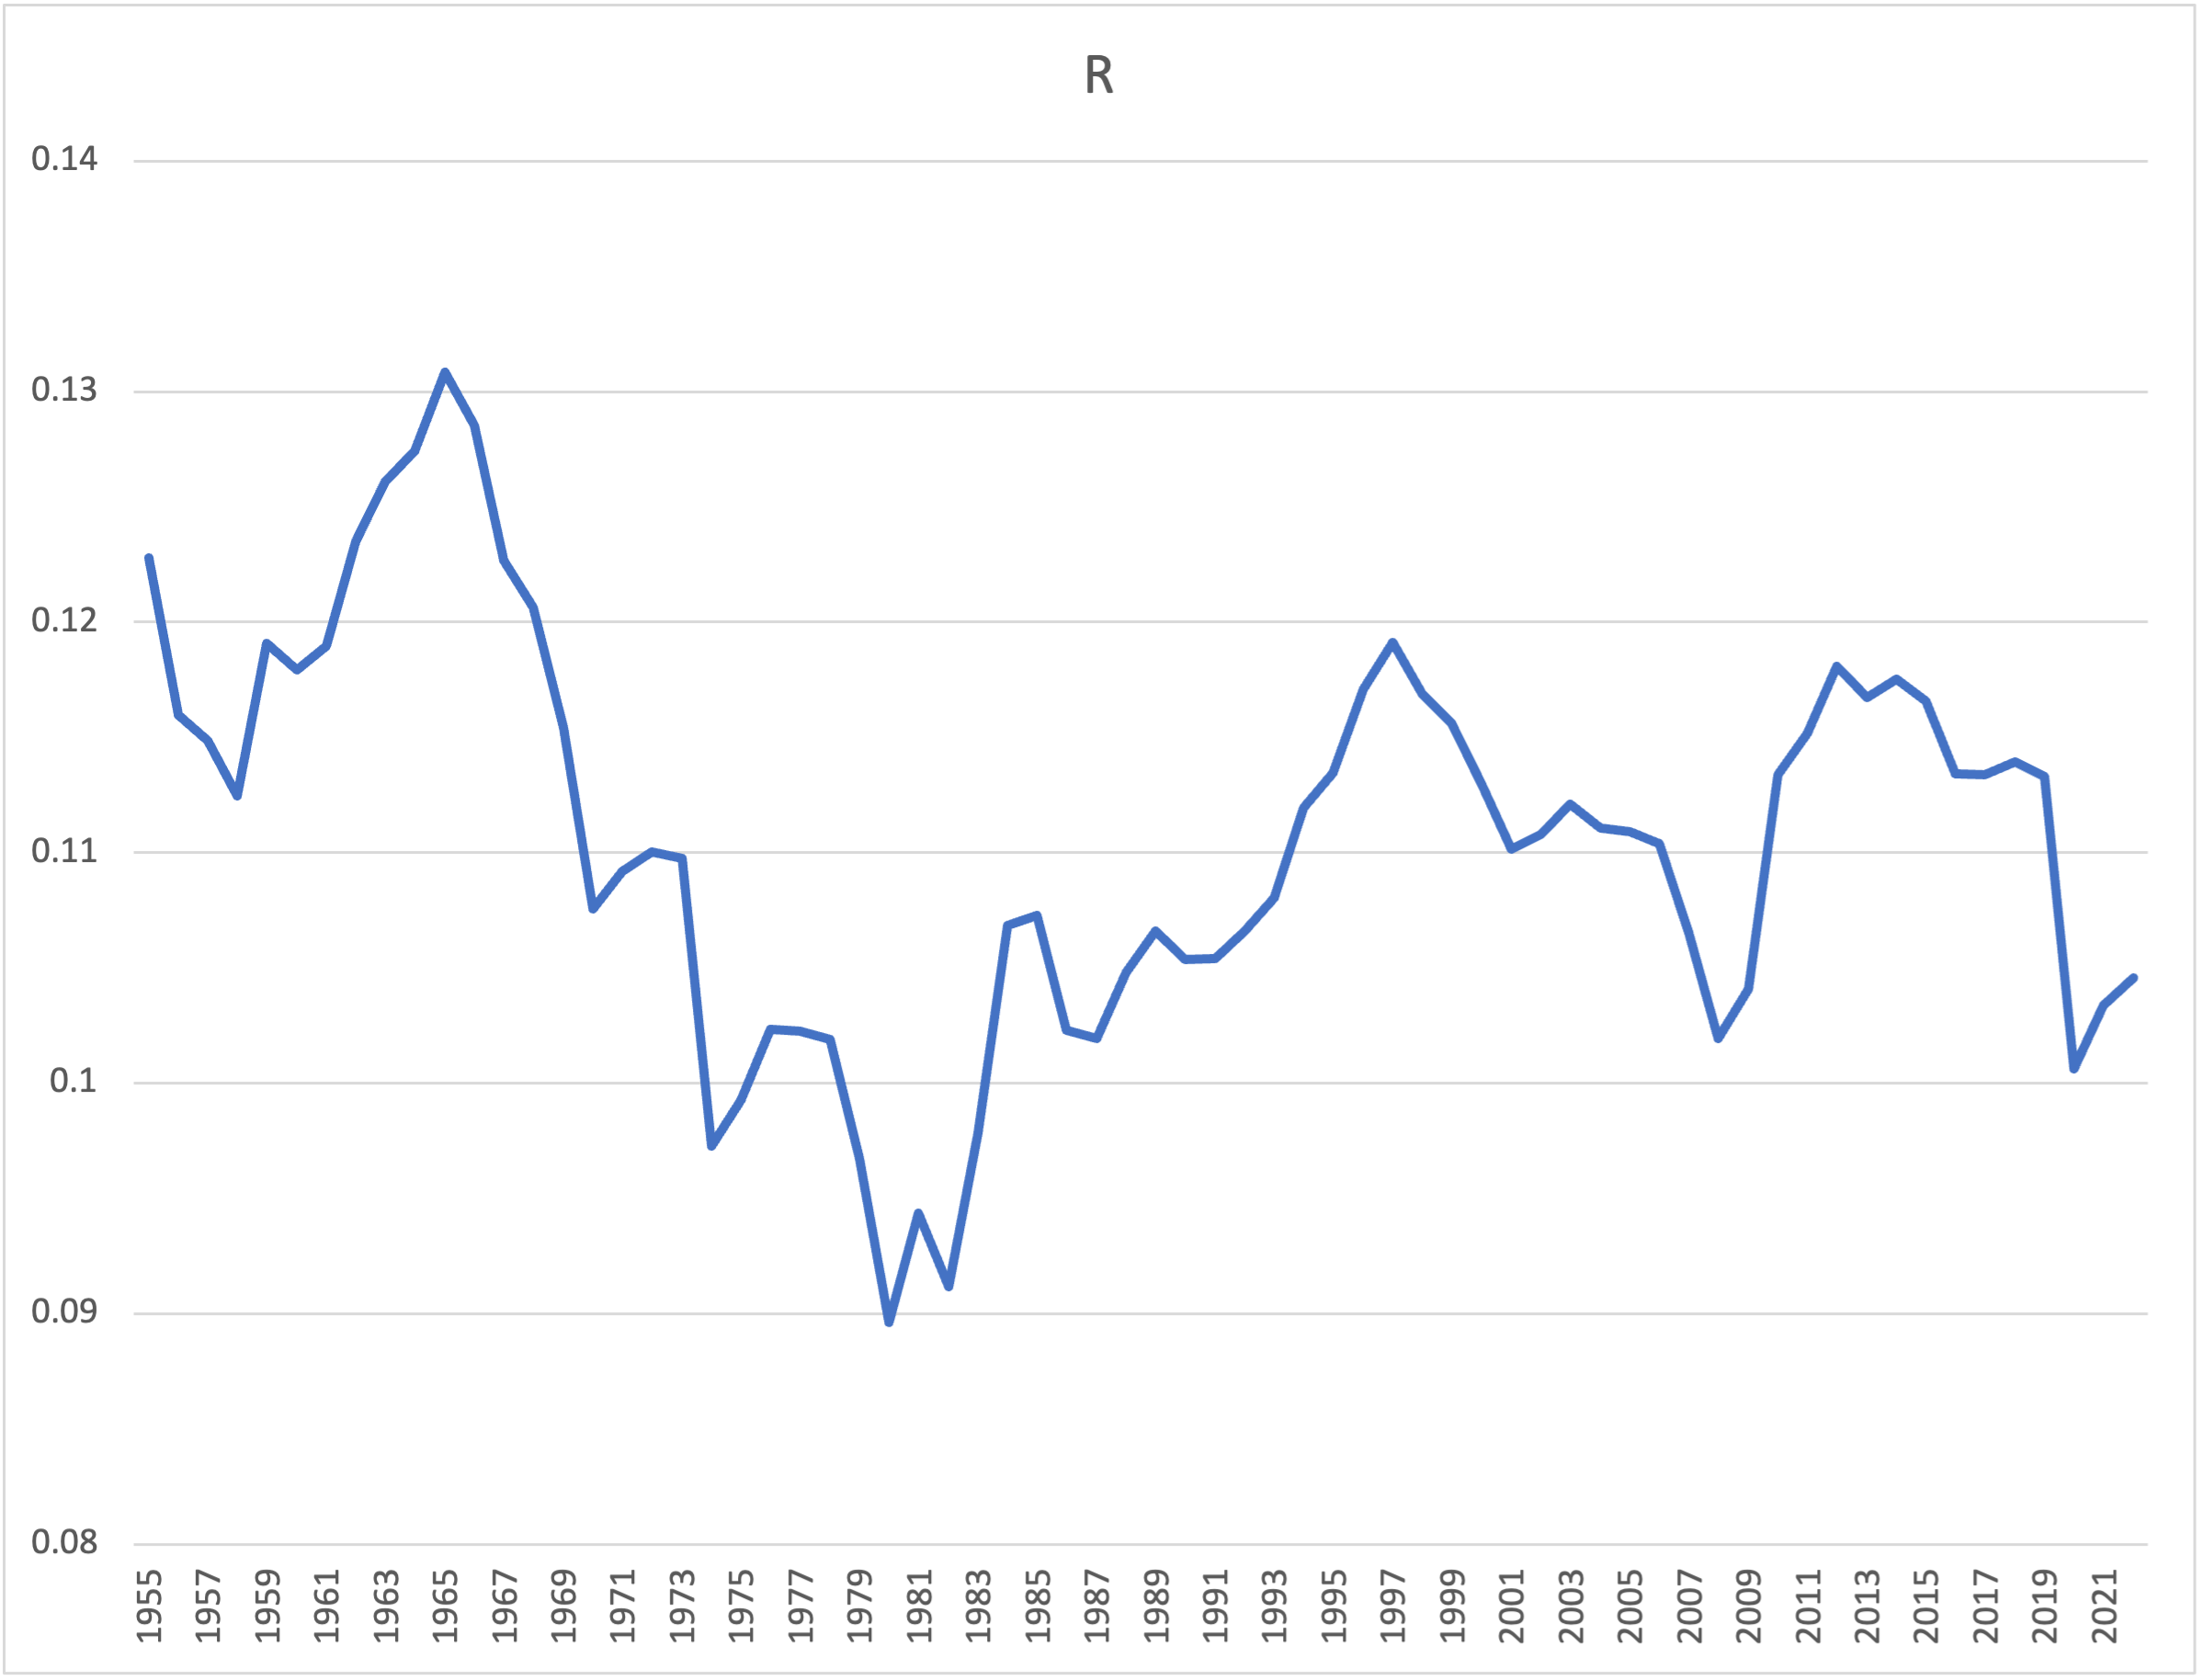
\includegraphics[width=0.6\textwidth]{graphs/r_usa.png}
            \caption{Return on Investment, US Economy
            \hyperlink{augmented_solow}{\beamergotobutton{Retour}}}
        \end{figure}
\end{frame}

\begin{frame}
    \frametitle{Kaldor's Stylized Facts}
    \hypertarget{wages}{} % Label for hyperlinks
    \framesubtitle{Wage Growth}
        \begin{figure}
            \centering
            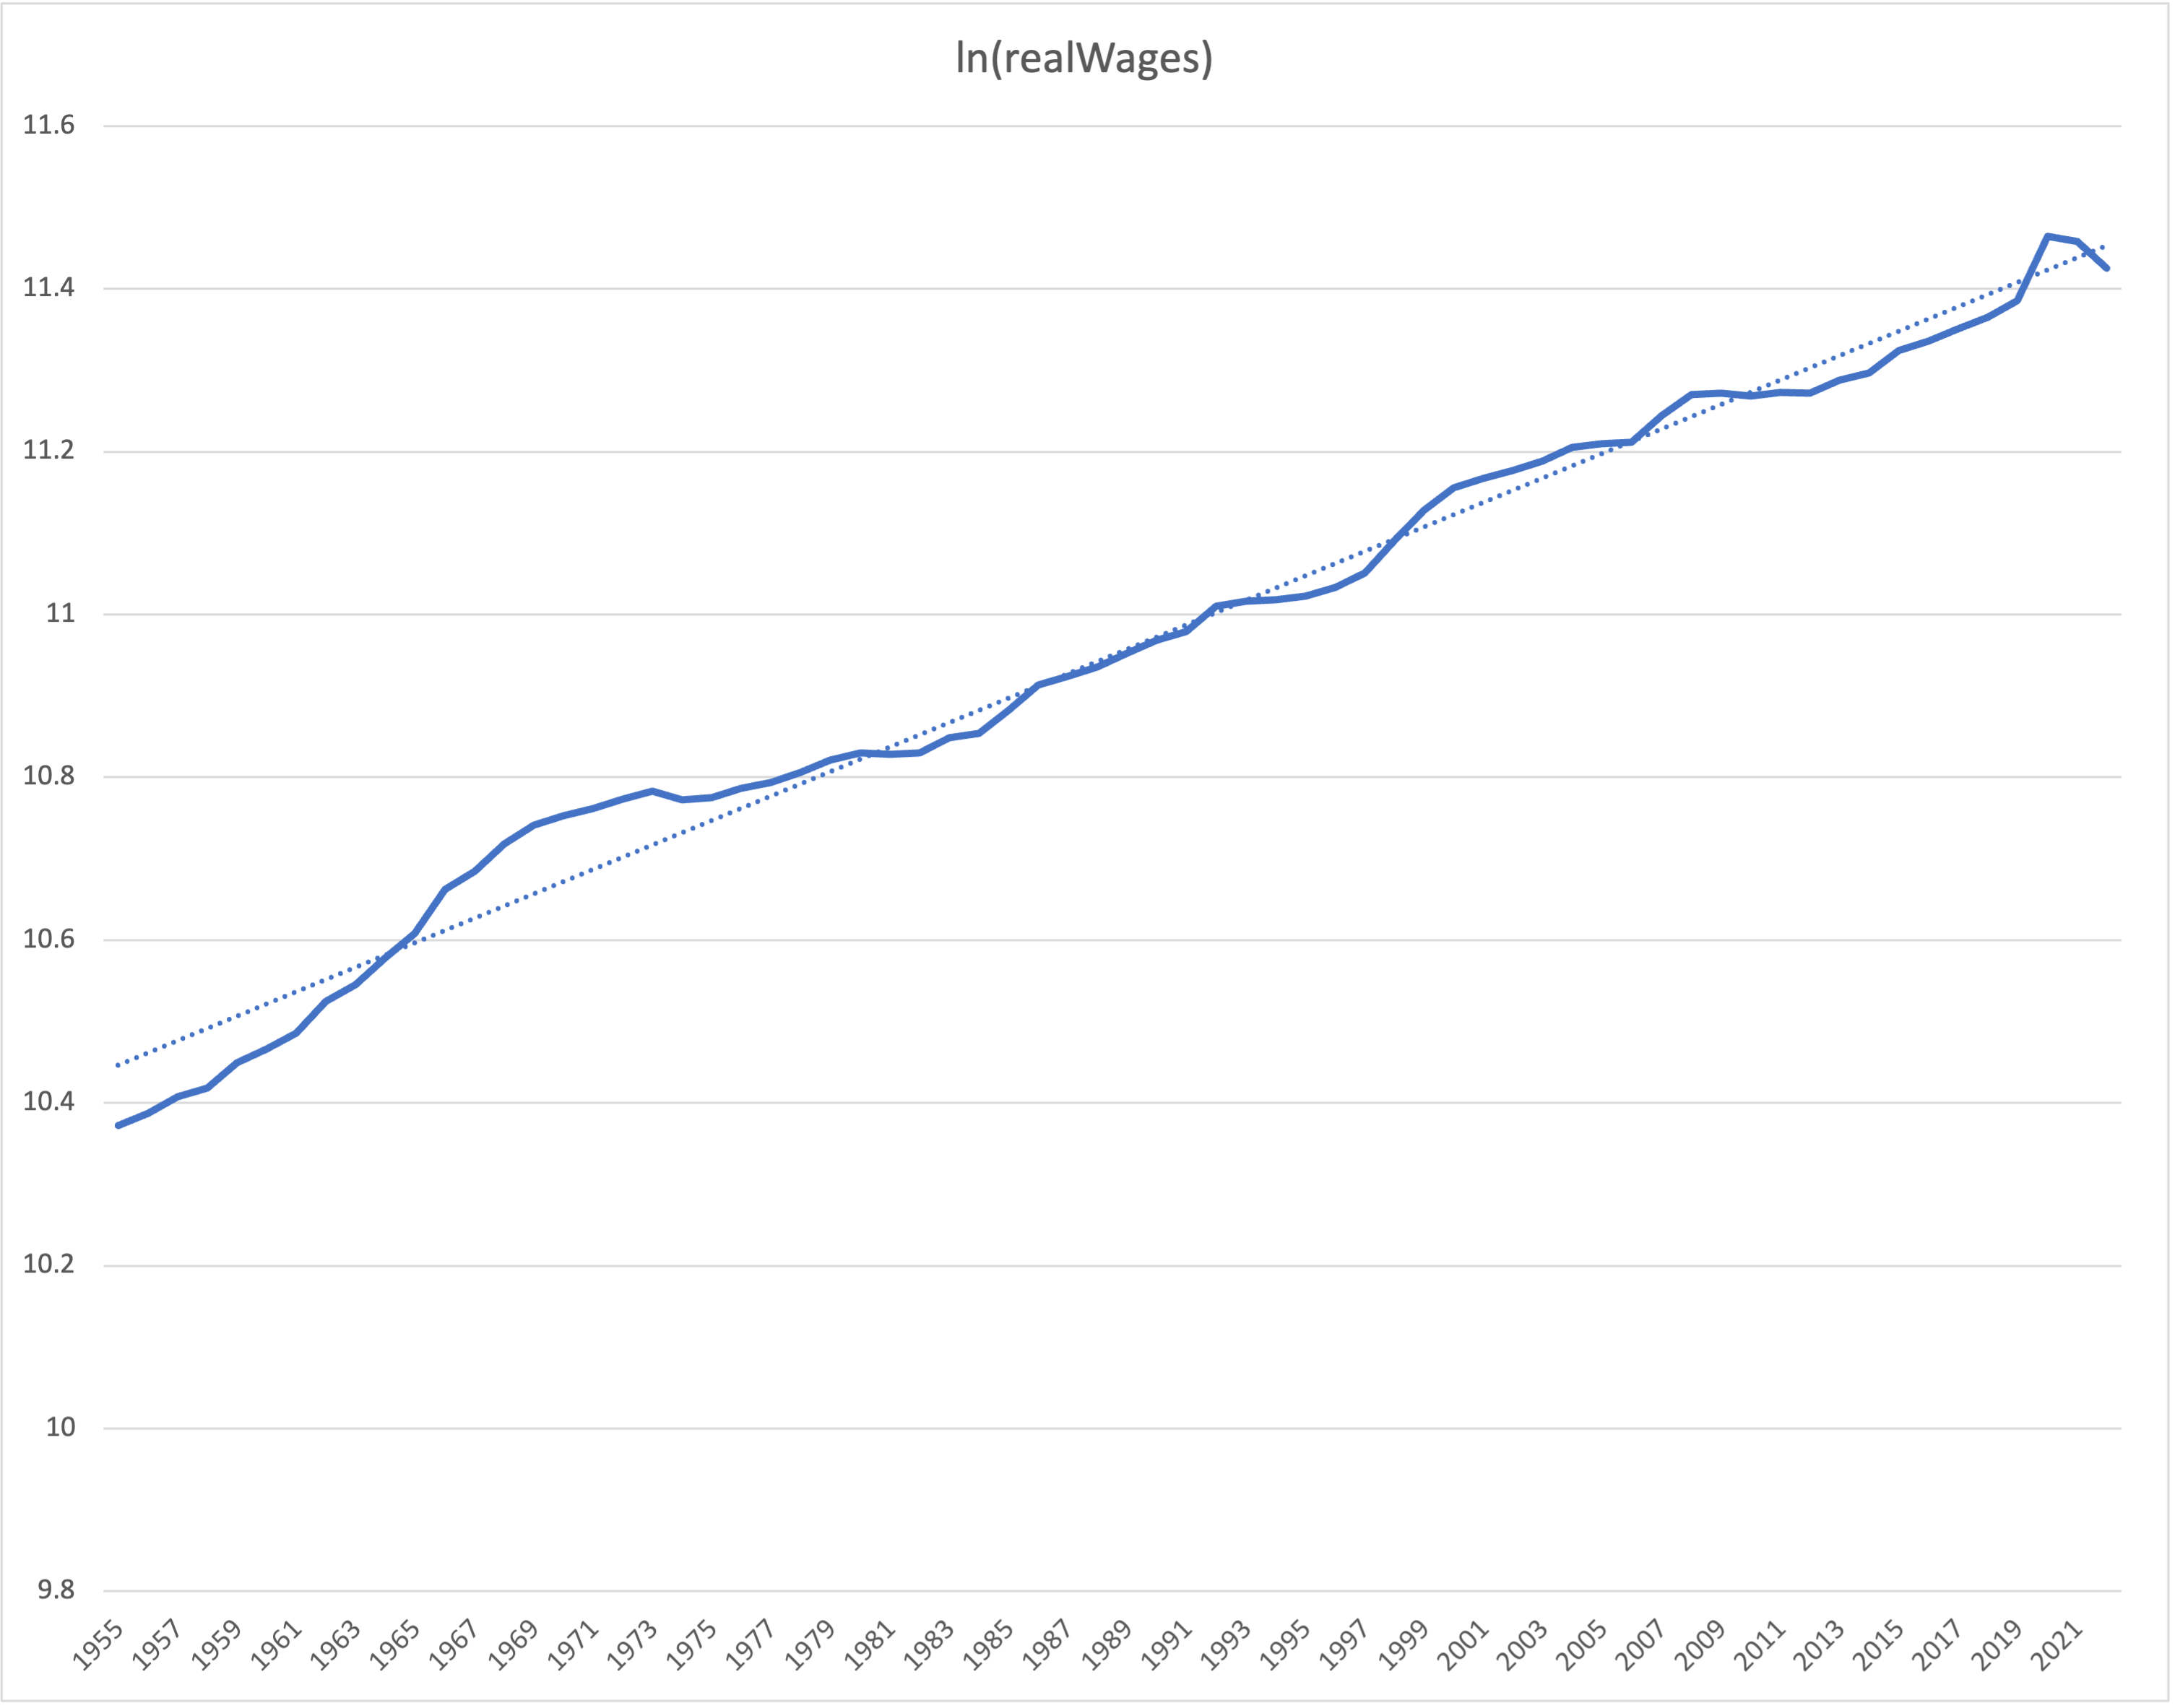
\includegraphics[width=0.6\textwidth]{graphs/lnwages_usa.png}
            \caption{Real wages, US Economy
            \hyperlink{augmented_solow}{\beamergotobutton{Retour}}}

        \end{figure}
\end{frame}

% \begin{frame}
%     \frametitle{Kaldor's Stylized Facts}
%     \hypertarget{return}{} % Label for hyperlinks
%     \framesubtitle{Taux de Rendement}
%         \begin{figure}
%             \centering
%             \includegraphics[width=0.8\textwidth]{graphs/}
%             \caption{Stability of Returns on Investment}
%         \end{figure}
% \end{frame}


\end{document}